\chapter{External Interface Requirements}
\label{chap:external_interfaces}

\section{User Interfaces}
\label{sec:ui}

\subsection{Web GUI}

The primary user interface is a single-page web application served at
\texttt{http://localhost:5000} (or the configured \texttt{PORT}).

\subsubsection{Layout Overview}

\begin{figure}[H]
  \centering
  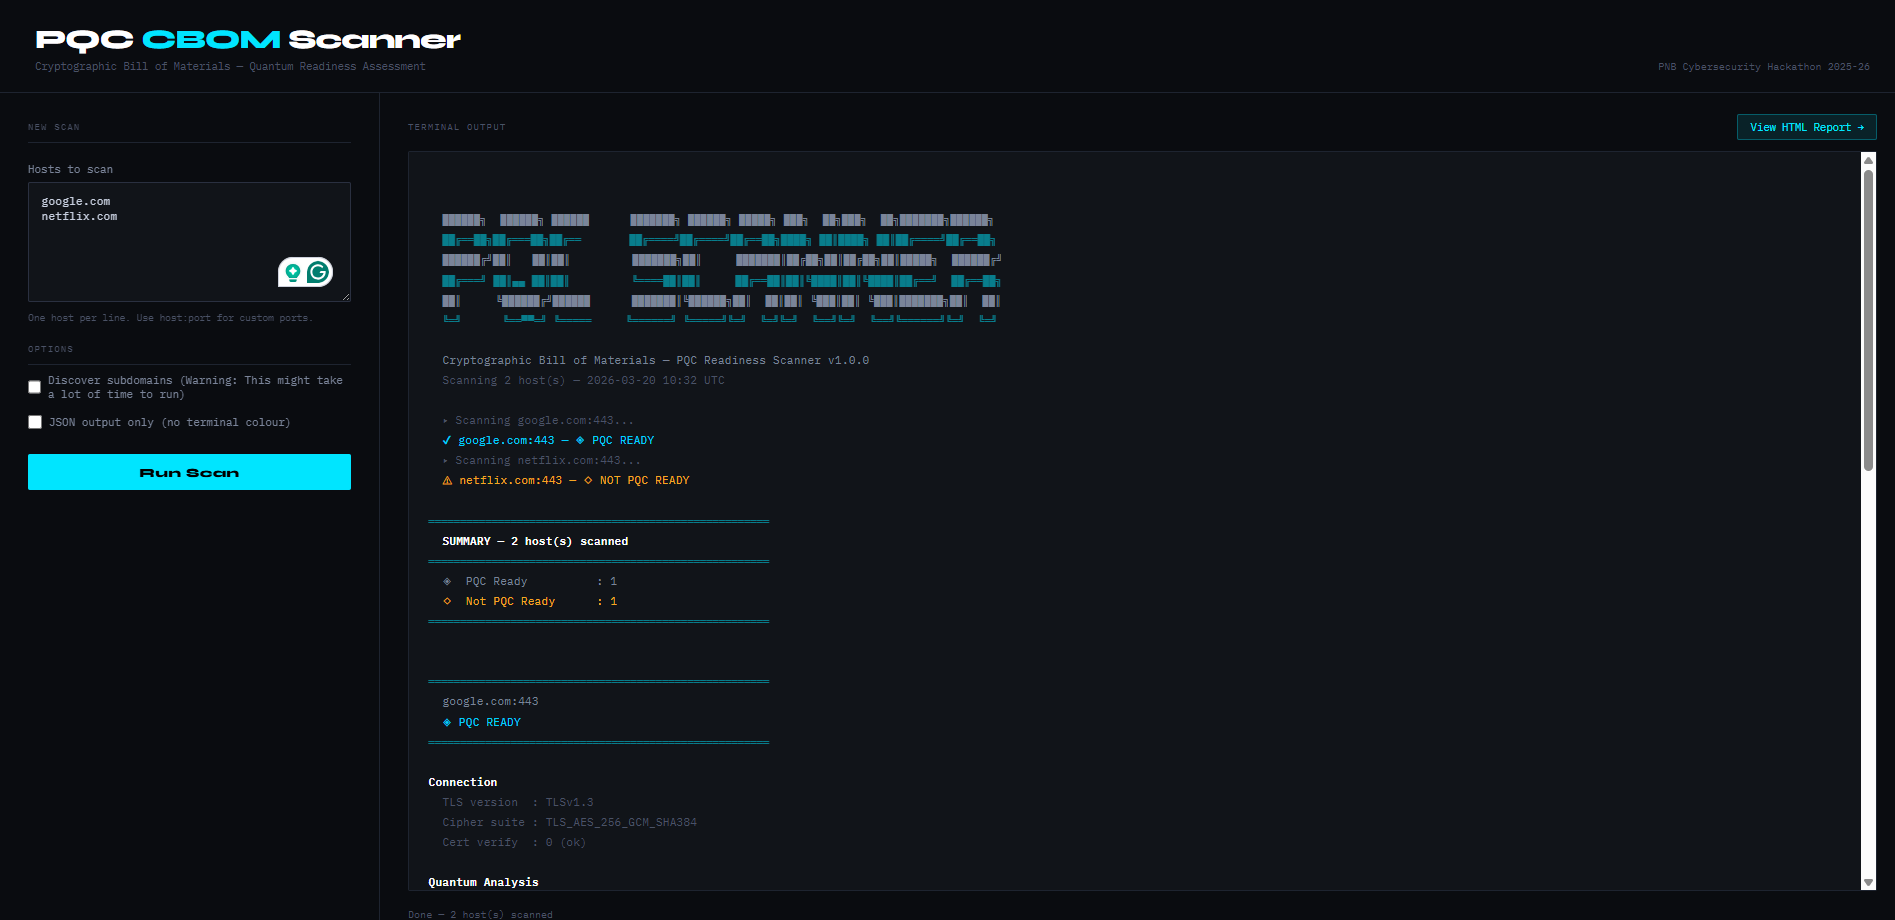
\includegraphics[width=\textwidth]{images/web_gui_full_output.png}
  \caption{Web GUI — Full layout: header, input panel (left), and output panel (right)}
  \label{fig:gui_full_layout}
\end{figure}

\noindent The page is divided into three regions:

\begin{description}[noitemsep, leftmargin=2cm]
  \item[Header] Application title (\textit{PQC CBOM Scanner}) with a cyan accent
    on \textit{CBOM}, subtitle, and hackathon context badge.
  \item[Left Panel (Input)] Host textarea, option checkboxes, Run Scan and Stop Scan
    buttons, version info footer.
  \item[Right Panel (Output)] Terminal-style scrollable output area with real-time
    SSE content, scan status spinner, and post-scan report link.
\end{description}

\subsubsection{Colour Scheme}

\begin{table}[H]
  \centering
  \caption{UI Colour Conventions}
  \label{tab:ui_colours}
  \begin{tabular}{L{4cm} L{3cm} L{7cm}}
    \toprule
    \textbf{Element} & \textbf{Hex Value} & \textbf{Usage} \\
    \midrule
    Background       & \texttt{\#0A0C10}  & Page and panel backgrounds. \\
    Cyan Accent      & \texttt{\#00E5FF}  & Headings, buttons, borders. \\
    Fully Quantum Safe & \texttt{\#00FF94} & FQS label, dots, text. \\
    PQC Ready        & \texttt{\#00BFFF}  & PQC label, dots, text. \\
    Not PQC Ready    & \texttt{\#F5A623}  & NOT label, warnings, dots. \\
    Critical         & \texttt{\#FF4D4D}  & CRIT label, errors, stop button. \\
    \bottomrule
  \end{tabular}
\end{table}

\subsubsection{Typography}

\begin{itemize}[noitemsep]
  \item \textbf{Syne} (Google Fonts) — used for headings and labels.
  \item \textbf{IBM Plex Mono} (Google Fonts) — used for monospace terminal
        output, code, and cipher names.
\end{itemize}

\subsection{HTML Report Interface}

\begin{figure}[H]
  \centering
  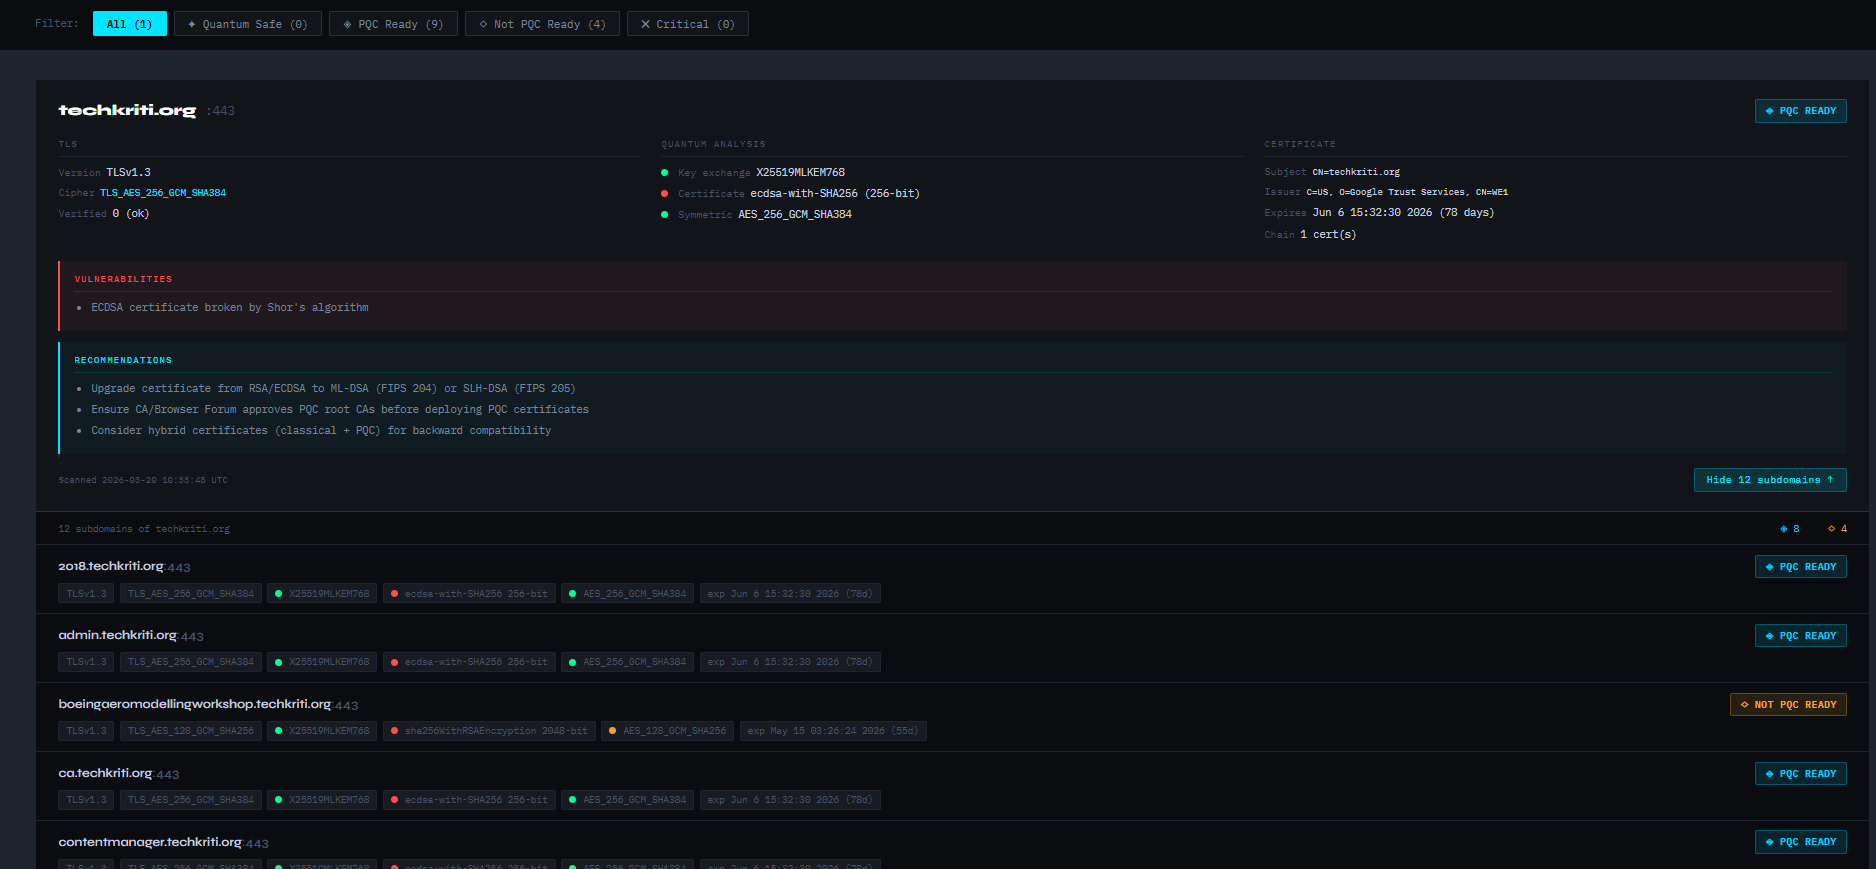
\includegraphics[width=\textwidth]{images/html_report_with_subdomain.png}
  \caption{HTML Report — Filter bar and domain group with subdomain drawer expanded}
  \label{fig:html_report_filter}
\end{figure}

The generated report provides the following interactive UI elements:

\begin{itemize}[noitemsep]
  \item \textbf{Sticky navigation bar} — Back to New Scan link and Download HTML
        button always visible while scrolling.
  \item \textbf{Statistics cells} — large numerals showing count and percentage
        per tier.
  \item \textbf{Progress bar} — colour-segmented horizontal bar.
  \item \textbf{Filter buttons} — toggle visibility of asset cards by tier.
  \item \textbf{Domain groups} — root asset card + collapsible subdomain drawer
        with compact subdomain rows.
  \item \textbf{Asset cards} — full CBOM detail per host with colour-coded
        indicator dots.
\end{itemize}

\subsection{Command-Line Interface}

The CLI scanner (\texttt{scan.sh}) accepts the following arguments:

\begin{table}[H]
  \centering
  \caption{CLI Arguments}
  \label{tab:cli_args}
  \begin{tabularx}{\textwidth}{L{3.5cm} L{10cm}}
    \toprule
    \textbf{Argument} & \textbf{Description} \\
    \midrule
    \texttt{<host>}          & One or more space-separated hostnames. \\
    \texttt{-f <file>}       & Read hosts from a plain-text file. \\
    \texttt{--subdomains}    & Enable Subfinder subdomain discovery. \\
    \texttt{--json}          & Output clean JSON; suppress ANSI codes. \\
    \texttt{--report}        & Generate an HTML report after scanning. \\
    \bottomrule
  \end{tabularx}
\end{table}

\section{Hardware Interfaces}
\label{sec:hardware_interfaces}

The application has no direct hardware interface requirements. It runs entirely
in software and communicates over standard Ethernet/Wi-Fi network interfaces via
the host OS's TCP/IP stack. No special hardware (HSM, SmartCard, etc.) is
required.

\section{Software Interfaces}
\label{sec:software_interfaces}

\begin{table}[H]
  \centering
  \caption{Software Interface Dependencies}
  \label{tab:software_interfaces}
  \begin{tabularx}{\textwidth}{L{3cm} L{2.5cm} L{8.5cm}}
    \toprule
    \textbf{Component} & \textbf{Version} & \textbf{Role} \\
    \midrule
    Python             & 3.11             & Application runtime. \\
    Flask              & $\geq$ 3.0       & HTTP framework; routes, SSE, template rendering. \\
    Gunicorn           & $\geq$ 21.0      & Production WSGI server (gthread worker). \\
    OpenSSL            & $\geq$ 3.0       & TLS handshake and certificate parsing via
                                           \texttt{s\_client}. \\
    Bash               & 5.x              & Scanner script (\texttt{scan.sh}); host
                                           loop, JSON assembly. \\
    Subfinder          & 2.13.0           & Passive/active subdomain enumeration. \\
    Docker             & $\geq$ 20.10     & Container packaging and runtime. \\
    \bottomrule
  \end{tabularx}
\end{table}

\section{Communication Interfaces}
\label{sec:communication_interfaces}

\begin{table}[H]
  \centering
  \caption{Communication Interfaces}
  \label{tab:comm_interfaces}
  \begin{tabularx}{\textwidth}{L{3.5cm} L{2.5cm} L{8cm}}
    \toprule
    \textbf{Interface} & \textbf{Protocol} & \textbf{Description} \\
    \midrule
    Browser $\leftrightarrow$ App & HTTP/1.1 & Form submission, page requests,
                                               report download. \\
    Browser $\leftarrow$ App (SSE) & HTTP/1.1 & Server-Sent Events stream of
                                                scan output lines. \\
    App $\rightarrow$ Target Hosts & TLS 1.3 (TCP/443) & Outbound TLS
                                                          handshake for
                                                          interrogation. \\
    App $\rightarrow$ Subfinder & STDIN/STDOUT & Local IPC pipe; domain input
                                                 and subdomain output. \\
    Subfinder $\rightarrow$ Internet & DNS / HTTPS & Queries public DNS resolvers
                                                      and certificate transparency
                                                      logs. \\
    \bottomrule
  \end{tabularx}
\end{table}

\noindent\textbf{Port assignments:}
\begin{itemize}[noitemsep]
  \item \texttt{5000/TCP} — Web GUI HTTP server (configurable via \texttt{PORT}
        env var).
  \item \texttt{443/TCP} — Default outbound port for TLS target connections
        (overridable per host).
\end{itemize}
